% Chapter 5

\chapter{État de l'art de la récupération du flux vidéo} % Main chapter title

\label{Chapter5} % For referencing the chapter elsewhere, use \ref{Chapter5}

%----------------------------------------------------------------------------------------

\section{Methodologie par la Webcam USB}

Nous nous aguérissons à l’utilisation de Video4Linux-utils, de plus nous avons trouvé
un journal en ligne expliquant la récupération du flux vidéo d’une webcam USB avec
V4L2-utils sur imx6. Dans un premier temps, nous avons capturé le flux d’une
webcam USB intégrée à un de nos ordinateurs personnels afin de comprendre les commandes
et paramètres. Ensuite nous avons récupéré une webcam USB lambda afin de tester les commandes
sur la carte openrex et essayer de capturer le retour vidéo. Une fois fonctionnel
nous passerons sur le flux vidéo de la Raspi Cam v2.

% \section{Commandes}
\begin{enumerate}
  \item Récupérer le port qui est connecté la webcam USB grâce à la commande :
  \textbf{lsusb -t}
%\begin{figure}[th]
%    \centering
%    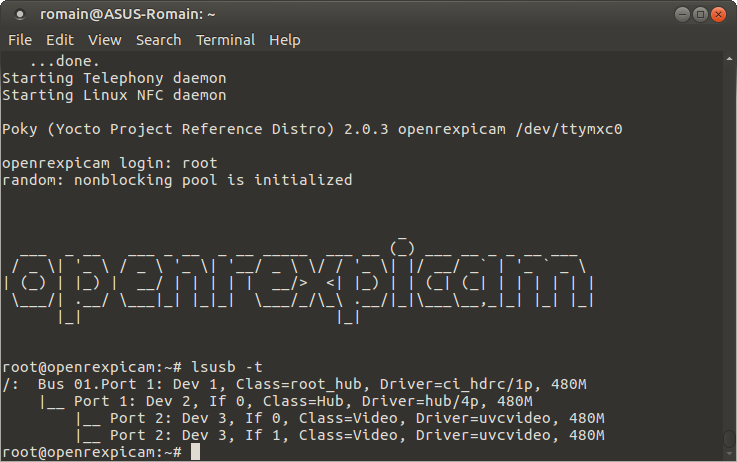
\includegraphics[width=1\linewidth,trim={0cm 0,6cm 0cm 12,5cm},clip]{webcam1.png}
%    \decoRule
%    \caption{Port USB de la webcam USB}  \label{fig:webcam1}
%\end{figure}

\item La webcam USB est sur le bus I2C n°1 avec comme identifiant de port 1.2.
%\begin{figure}[th]
%    \centering
%    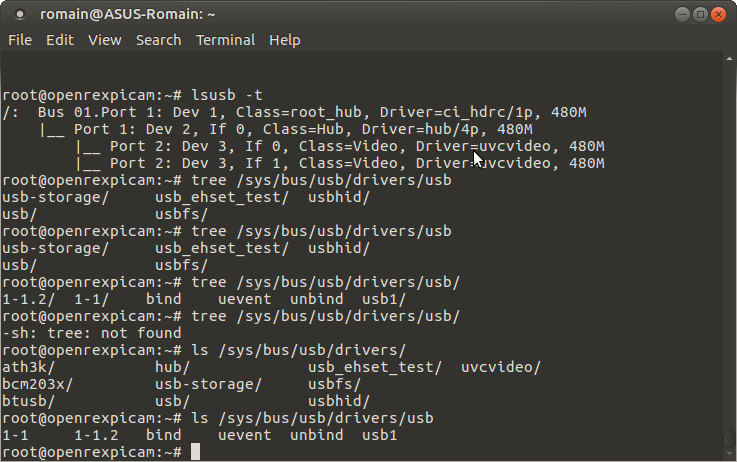
\includegraphics[width=1\linewidth,trim={0cm 0,6cm 0cm 14,5cm},clip]{webcam2.png}
%    \decoRule
%    \caption{Vérification du port et identifiant de la webcam USB}  \label{fig:webcam2}
%\end{figure}

\item Il est nécessaire d'écrire le numéro du bus et l’identifiant du port dans les fichiers bind
et unbind. Le fichier bind permet de  « lier » un appareil USB à son driver et
ainsi le rendre visible pour le système tandis que le fichier unbind lui détache
le driver de son appareil USB pour le « cacher » du système.
%\begin{figure}[th]
%    \centering
%    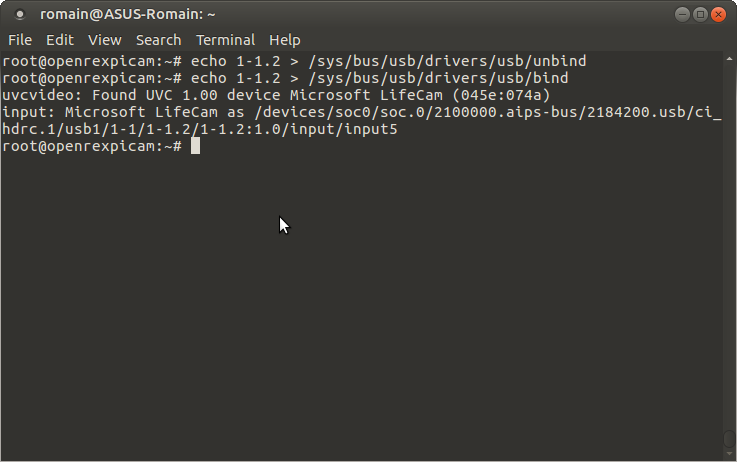
\includegraphics[scale=0.5,trim={0cm 11,5cm 0cm 1,9cm},clip]{webcam3.png}
%    \decoRule
%    \caption{Liaison entre la webcam USB et son driver}  \label{fig:webcam3}
%\end{figure}

\item La webcam USB est bien reconnu par notre système qui affiche sa
référence %(cf. Figure \ref{fig:webcam3}).

\item Démarrer un flux vidéo sur notre webcam USB s'effectue avec la commande :
\textbf{\# gst-launch-1.0 v4l2src device="/dev/video0" ! video/x-raw,w
idth=640,height=480 ! autovideosink}

%\begin{figure}[th]
%    \centering
%    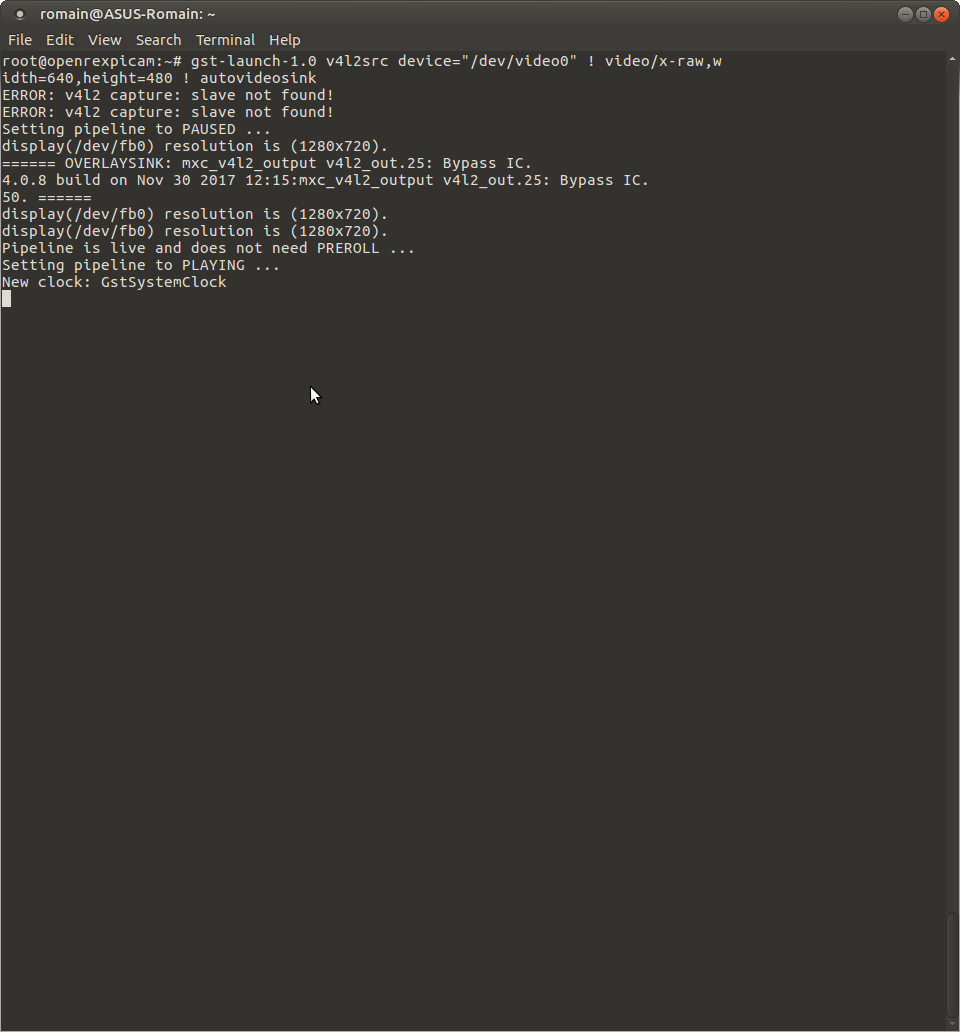
\includegraphics[scale=0.4,trim={0cm 26,1cm 0cm 1,7cm},clip]{webcam4.png}
%    \decoRule
%    \caption{Capture du flux vidéo de la webcam USB}  \label{fig:webcam4}
%\end{figure}

\item Nous sommes persuadés de la bonne capture du flux vidéo puisque lorsque
nous la lançons, le retour de la commande se fige à :

\begin{lstlisting}
New clock GstSystemClock
\end{lstlisting}

C'est exactement le même endroit quand nous lançons la même commande sur notre
propre ordinateur avec notre webcam intégrée. De plus une petite LED verte s’allume
au moment de l’envoi de cette commande (cf. Figure \ref{fig:webcam5}).
%\begin{figure}[th]
%    \centering
%    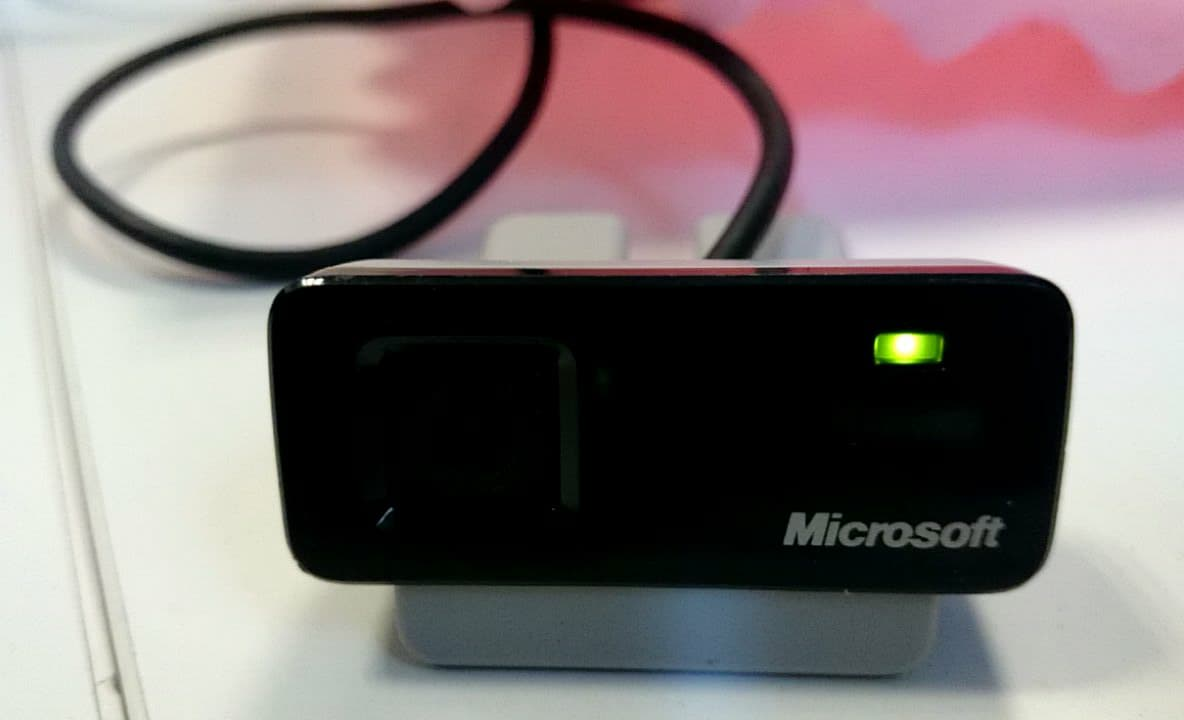
\includegraphics[scale=0.15,trim={10cm 2cm 4cm 9,5cm},clip]{webcam5.png}
%    \decoRule
%    \caption{LED verte allumée lors de l'envoi de la commande}  \label{fig:webcam5}
%\end{figure}

\end{enumerate}

\section{Problèmes}

Notre principal problème pour l’instant est de récupérer ce flux vidéo puisqu’il
est impossible de l’afficher directement dans le terminal, pour tester cela nous
essayons de l’afficher sur nos ordinateurs par le réseau WiFi en protocole UDP.

\section{Point d'amélioration}

Pour commencer il est nécessaire de mettre l’image de l'openrex à jour afin de se
connecter à un réseau WiFi ensuite récupérer ce flux vidéo par le réseau WiFi sur
nos ordinateurs en UDP.

Finalement une fois que nous aurons réussi à afficher le flux vidéo de la webcam
USB sur nos ordinateurs nous essayerons d’effectuer le même processus mais pour
la Raspi Cam v2, qui se pilote par le CSI et non l’USB.

\section{Sources}

Lien du blog de la récupération du flux vidéo par la webcam USB :

\href{http://jas-hacks.blogspot.fr/2014/04/imx6-gstreamer-imx-and-usb-webcam.html}
{http://jas-hacks.blogspot.fr/2014/04/imx6-gstreamer-imx-and-usb-webcam.html}
